\section{Программная реализация}

В рамках лабораторной работы вычислительный модуль был реализован в виде настольного приложения на языке C\# с использованием платформы .NET~9 и библиотеки Windows Forms. Приложение объединяет ввод данных, приведение задачи к каноническому виду, решение симплекс-методом и проведение вычислительного эксперимента в единой интерактивной среде.

\subsection{Структура приложения}

Программа состоит из нескольких логических модулей:

\begin{itemize}
    \item модуль описания задачи линейного программирования, содержащий коэффициенты целевой функции, ограничения и условия на переменные;
    \item модуль преобразования исходной задачи к каноническому виду, включая обработку свободных переменных, ограничений типа $\leq$, $\geq$ и $=$, а также формирование искусственного базиса;
    \item модуль двухфазного симплекс-метода, выполняющий поиск допустимого базисного решения и последующее нахождение оптимума;
    \item модуль вычислительного эксперимента, который автоматически возмущает правые части ограничений и рассчитывает статистики абсолютной и относительной погрешностей;
    \item графический интерфейс пользователя, обеспечивающий ввод данных и визуализацию результатов.
\end{itemize}

\subsection{Пользовательский интерфейс}

Главное окно программы содержит две вкладки:

\begin{itemize}
    \item \textbf{``Решение задачи''} --- для задания размерности задачи, ввода коэффициентов, выбора типа ограничений и просмотра найденного решения;
    \item \textbf{``Вычислительный эксперимент''} --- для запуска серии экспериментов с возмущением правых частей и анализа полученных ошибок в табличной и графической форме.
\end{itemize}

На первой вкладке пользователь может изменять число переменных и ограничений, редактировать таблицу коэффициентов целевой функции, задавать знаки ограничений и типы переменных (\texttt{free} или $\geq 0$). После нажатия кнопки \textbf{``Решить задачу''} в окне отображаются:

\begin{itemize}
    \item статус решения и найденное оптимальное значение целевой функции;
    \item значения исходных переменных;
    \item каноническая форма задачи, построенная программой;
    \item перечень выполненных преобразований;
    \item журнал итераций двухфазного симплекс-метода.
\end{itemize}

\begin{figure}[h]
   \centering
   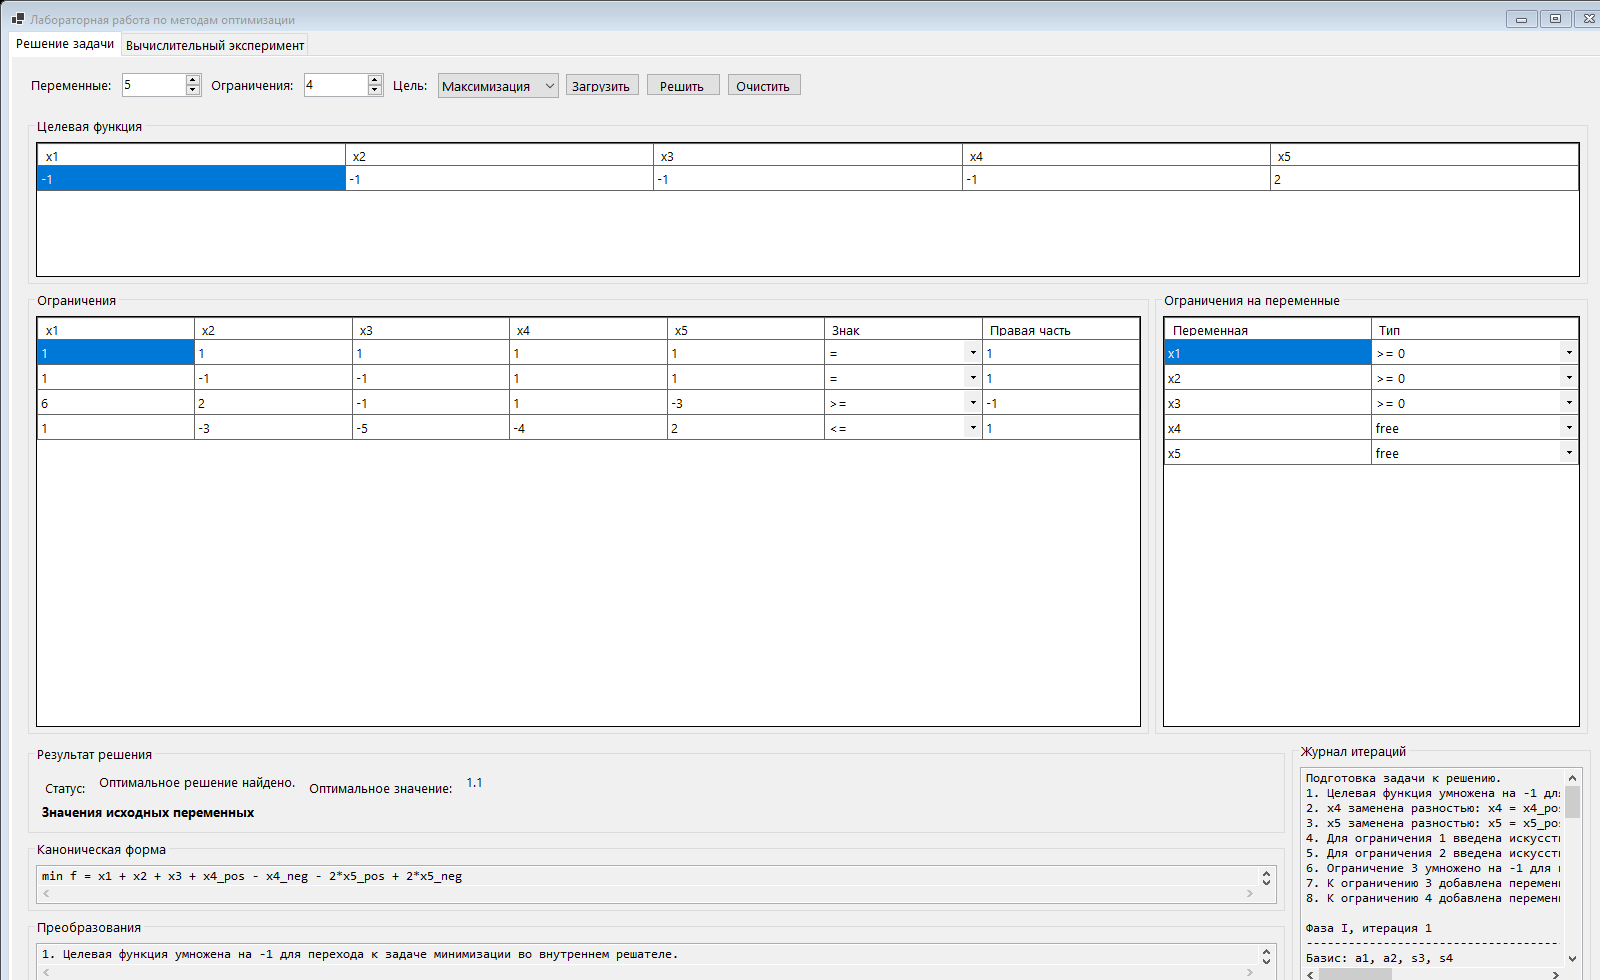
\includegraphics[width=0.98\textwidth]{ui_main.png}
   \caption{Главное окно программы, реализованной на C\# с интерактивным пользовательским интерфейсом.}
   \label{fig:ui-main}
\end{figure}

\subsection{Сценарий работы пользователя}

Типовой порядок работы с программой состоит из следующих шагов:

\begin{enumerate}
    \item задать число переменных и ограничений;
    \item ввести коэффициенты целевой функции и матрицы ограничений;
    \item указать знак каждого ограничения и тип каждой переменной;
    \item запустить решение задачи;
    \item проанализировать найденное решение, каноническую форму и журнал итераций;
    \item при необходимости перейти на вкладку вычислительного эксперимента и исследовать влияние возмущений на точность результата.
\end{enumerate}

Таким образом, графический интерфейс делает программную реализацию лабораторной работы наглядной и удобной для повторных вычислений, а также сокращает вероятность ошибок при ручном вводе исходных данных.
